\chapter{Considerações finais}
\label{consideracoes-finais}


\section{Resultados Prelimirares}
\label{results}

\subsection{Plugin Ldap UnB}

O \textit{plugin} que faz comunicação com o Ldap da UnB encontra-se em fase de homolagação
Com o auxilio de uma ferramenta de análise de código para \textit{Ruby} chamada Rcov, foi obtida a taxa de cobertura de código do plugin desenvolvido, além de alguns dados sobre a execução dos testes funcionais e unitários que seguem abaixo:

\begin{itemize}
\item Quantidade de testes executados: \textbf{96 testes;}
\item Quantidade de assertivas executadas: \textbf{111 assertivas;}
\item Quantiadde de falhas obtidas: \textbf{0 falhas;}
\item Tempo de execução dos testes: \textbf{7.8 segundos;}
\end{itemize}

Na imagem abaixo existem dois gráficos de cobertura de codigo, o primeiro definido como \textit{'total coverage'} representa a contagem realizada com as linhas em branco e os comentários do código, já o \textit{'code coverage'} representa a contagem realizada sem as linhas em branco e os comentários do código.

%
\begin{figure}[!h]
    \centering
    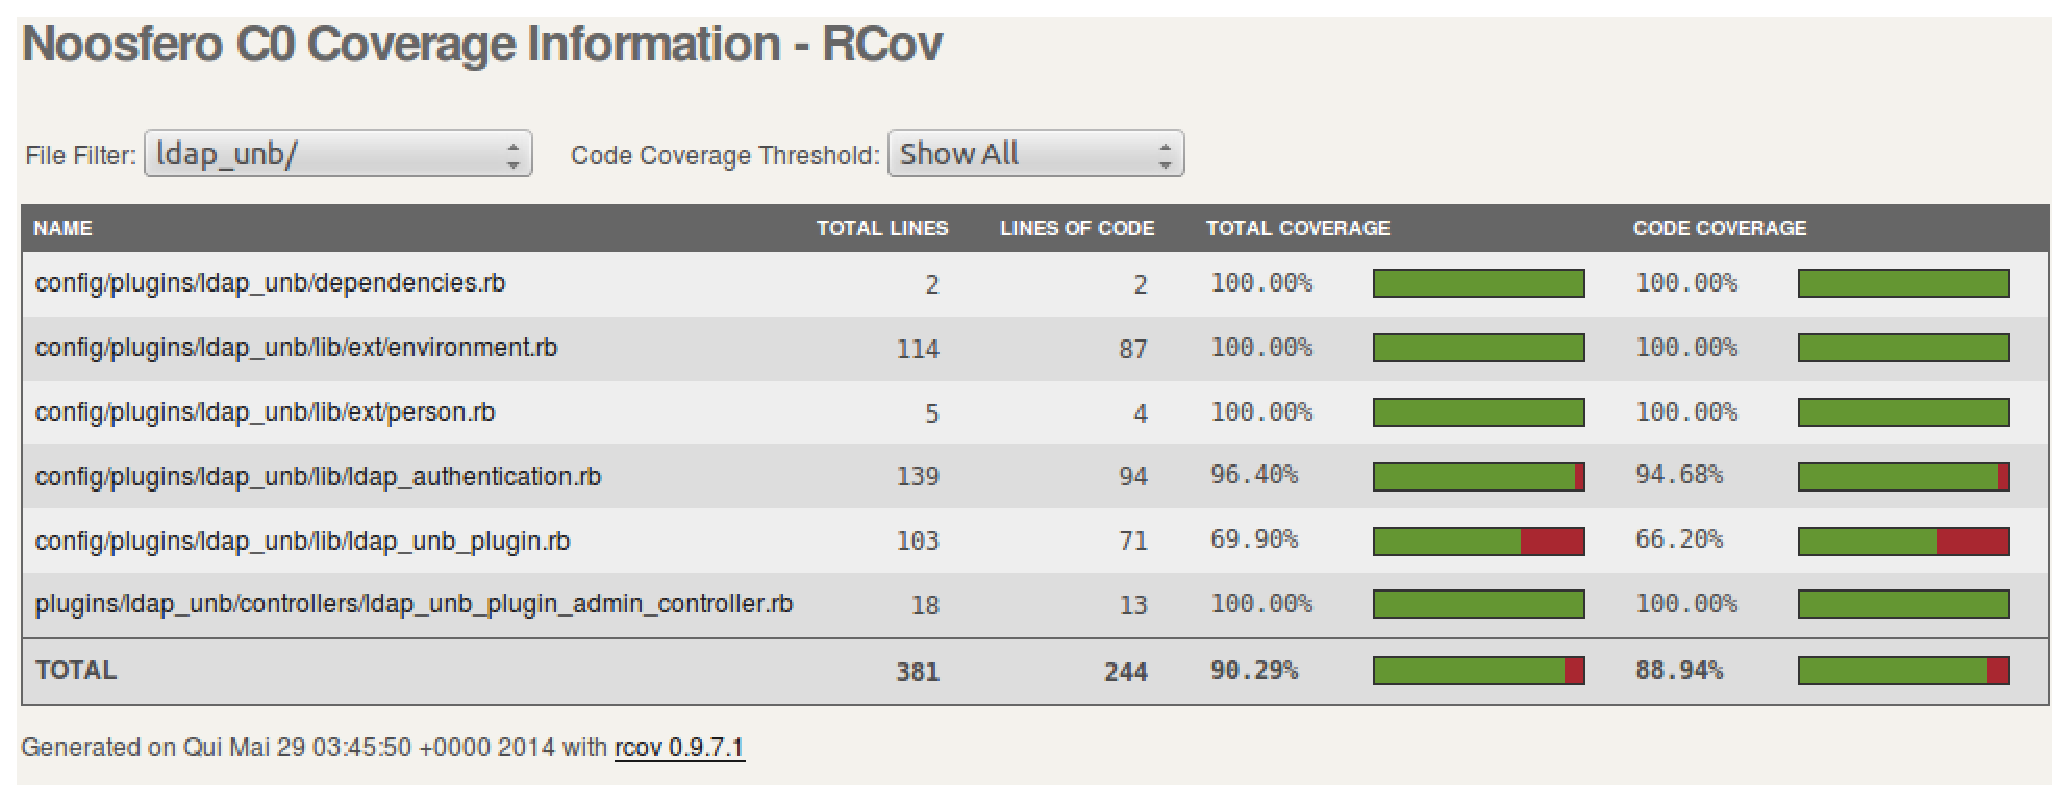
\includegraphics[keepaspectratio=false,scale=0.45]
      {figuras/cobertura_teste.eps}
    \caption{Cobertura de código do Plugin LdapUnb}
    \label{consideracoes_cobertura1}
\end{figure}
%

\subsection{Plugin para envio de TCC}

A ferramenta Rcov também foi utilizada para dimensionar a taxa de cobertura de código deste plugin, segue os dados sobre a execução dos testes funcionais e unitários:
\begin{itemize}
\item Quantidade de testes executados: \textbf{28 testes};
\item Quantidade de assertivas executadas: \textbf{84 assertivas};
\item Quantiadde de falhas obtidas: \textbf{0 falhas};
\item Tempo de execução dos testes: \textbf{10,5 segundos};
\end{itemize}

Na imagem abaixo está representado a cobertura de código, extraída da ferramenta Rcov:

\begin{figure}[!h]
    \centering
    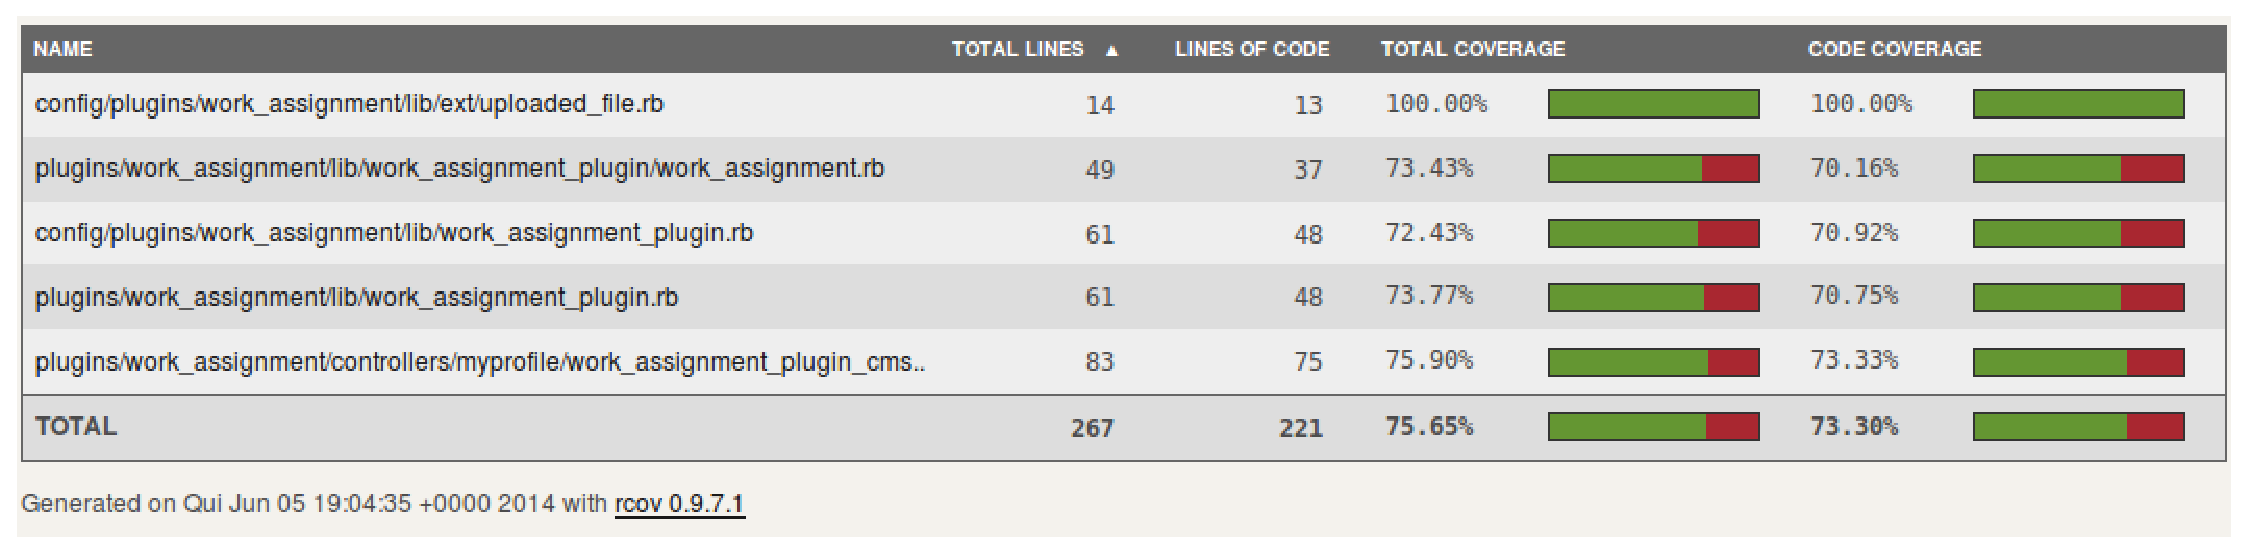
\includegraphics[keepaspectratio=false,scale=0.45]
      {figuras/cobertura_tcc.eps}
    \caption{Cobertura de código do Plugin para envio de TCC}
    \label{consideracoes_cobertura2}
\end{figure}

Para este plugin também foram desenvolvidos testes automáticos de aceitação, afim de validar a experiência do usuário em diferentes cenários possiveis:
\begin{itemize}
\item Quantidade de cenários executados: \textbf{6 cenários};
\item Quantidade de passos executadas: \textbf{130 passos};
\item Quantiadde de falhas obtidas: \textbf{0 falhas};
\item Tempo de execução dos testes: \textbf{7 minutos e 18 segundos};
\end{itemize}

IMAGEM

\section{Próximos Passos}

Aplicar as técnicas de usabilidade pesquisadas durante o trabalho, em um processo baseado em BDD e TDD, a fim de verificar problemas de usabilidade, e satisfação e uso.

Verificar os padrões de design  e usabilidade adotados pelo Noosfero e propor melhorias de usabilidade.

\subsection{Portal do Software Público}
\subsection{Cronograma}